\documentclass[../main.tex]{subfiles}
\begin{document}

	\chapter{Finite element basis functions}
	\label{chap:chap_3}
	\noindent The specific basis functions exemplified in Section \hyperref[chap:chap_2]{2} are in general nonzero on the entire domain $\Omega$, see Figure \hyperref[fig:img_13]{13} for an example where we plot $\psi_{0}(x)=\sin \frac{1}{2} \pi x$ and $\psi_{1}(x)=\sin 2 \pi x$ together with a possible sum $u(x)=4 \psi_{0}(x)-\frac{1}{2} \psi_{1}(x)$. We shall now turn the attention to basis functions that have compact support, meaning that they are nonzero on only a small portion of $\Omega$. Moreover, we shall restrict the functions to be \textit{piecewise polynomials}. This means that the domain is split into subdomains and the function is a polynomial on one or more subdomains, see Figure \hyperref[fig:img_14]{14} for a sketch involving locally defined hat functions that make $u=\sum_{j} c_{j} \psi_{j}$ piecewise linear. At the boundaries between subdomains one normally forces continuity of the function only so that when connecting two polynomials from two subdomains, the derivative becomes discontinuous. These type of basis functions are fundamental in the finite element method.
	\begin{figure}[H]
		\centering
		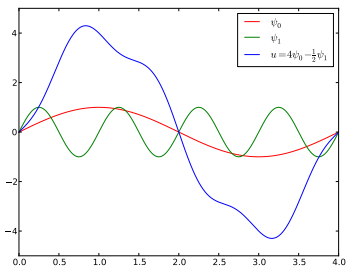
\includegraphics[width=0.7\linewidth]{img_13}
		\caption{A function resulting from adding two sine basis functions.}
		\label{fig:img_13}
	\end{figure}
	We first introduce the concepts of elements and nodes in a simplistic fashion
	as often met in the literature. Later, we shall generalize the concept of an
	element, which is a necessary step to treat a wider class of approximations within
	the family of finite element methods. The generalization is also compatible with
	the concepts used in the \href{https://fenicsproject.org/}{FEniCS} finite element software
	\section[Elements and nodes]{Elements and nodes}
	\label{sec:sec_3_1}
	Let us divide the interval $\Omega$ on which $f$ and $u$ are defined into non-overlapping subintervals $\Omega^{(e)}, e=0, \ldots, N_{e}$ :
	\begin{equation}\label{eqa51}
		\Omega=\Omega^{(0)} \cup \cdots \cup \Omega^{\left(N_{c}\right)}.
	\end{equation}
	We shall for now refer to $\Omega^{(e)}$ as an element, having number $e$. On each element we introduce a set of points called nodes. For now we assume that the nodes are uniformly spaced throughout the element and that the boundary points of the elements are also nodes. The nodes are given numbers both within an element and in the global domain. These are referred to as \textit{local} and \textit{global} node numbers, respectively. Figure \hyperref[fig:img_15]{15} shows element boundaries with small vertical lines, nodes as small disks, element numbers in circles, and global node numbers under the nodes.
	
	Nodes and elements uniquely define a \textit{finite element mesh}, which is our discrete representation of the domain in the computations. A common special
	\begin{figure}[H]
		\centering
		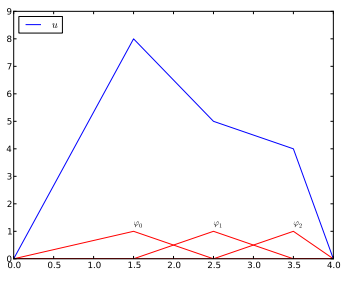
\includegraphics[width=0.7\linewidth]{img_14}
		\caption{A function resulting from adding three local piecewise linear (hat)
			functions.}
		\label{fig:img_14}
	\end{figure}
	\begin{figure}[H]
		\centering
		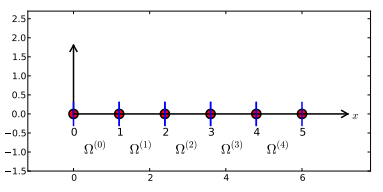
\includegraphics[width=0.7\linewidth]{img_15}
		\caption{Finite element mesh with 5 elements and 6 nodes.}
		\label{fig:img_15}
	\end{figure}
	
	\noindent case is that of a \textit{uniformly partitioned mesh} where each element has the same
	length and the distance between nodes is constant.
	
	\noindent \textbf{Example.} $\quad$ On $\Omega=[0,1]$ we may introduce two elements, $\Omega^{(0)}=[0,0.4]$ and $\Omega^{(1)}=[0.4,1]$. Furthermore, let us introduce three nodes per element, equally spaced within each element. Figure \hyperref[fig:img_16]{16} shows the mesh. The three nodes in element number 0 are $x_{0}=0, x_{1}=0.2$, and $x_{2}=0.4$. The local and global node numbers are here equal. In element number 1 , we have the local nodes $x_{0}=0.4$, $x_{1}=0.7$, and $x_{2}=1$ and the corresponding global nodes $x_{2}=0.4, x_{3}=0.7$, and $x_{4}=1$. Note that the global node $x_{2}=0.4$ is shared by the two elements.
	\begin{figure}[H]
		\centering
		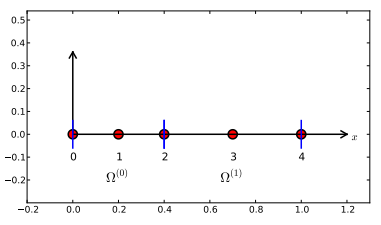
\includegraphics[width=0.7\linewidth]{img_16}
		\caption{Finite element mesh with 2 elements and 5 nodes.}
		\label{fig:img_16}
	\end{figure}
	
	For the purpose of implementation, we introduce two lists or arrays: \mycode{nodes}
	for storing the coordinates of the nodes, with the global node numbers as indices,
	and \mycode{elements} for holding the global node numbers in each element, with the
	local node numbers as indices. The \mycode{nodes} and \mycode{elements} lists for the sample
	mesh above take the form
	\begin{lstlisting}[numbers=none]
		nodes = [0, 0.2, 0.4, 0.7, 1]
		elements = [[0, 1, 2], [2, 3, 4]]	
	\end{lstlisting}
	Looking up the coordinate of local node number 2 in element 1 is here done by
	\mycode{nodes[elements[1][2]]} (recall that nodes and elements start their numbering
	at 0).
	
	The numbering of elements and nodes does not need to be regular. Figure \hyperref[fig:img_17]{17}
	shows and example corresponding to
	\begin{lstlisting}[numbers=none]
		nodes = [1.5, 5.5, 4.2, 0.3, 2.2, 3.1]
		elements = [[2, 1], [4, 5], [0, 4], [3, 0], [5, 2]]	
	\end{lstlisting}
	\section[The basis functions]{The basis functions}
	\label{sec:sec_3_2}
	\noindent \textbf{Construction principles}. Finite element basis functions are in this text recognized by the notation $\varphi_{i}(x)$, where the index now in the beginning corresponds to a global node number. In the current approximation problem we shall simply take $\psi_{i}=\varphi_{i}$.
	
	Let $i$ be the global node number corresponding to local node $r$ in element number $e$. The finite element basis functions $\varphi_{i}$ are now defined as follows.
	\begin{figure}[H]
		\centering
		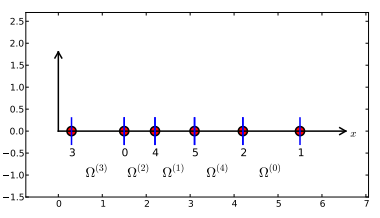
\includegraphics[width=0.7\linewidth]{img_17}
		\caption{Example on irregular numbering of elements and nodes.}
		\label{fig:img_17}
	\end{figure}
	
	\begin{itemize}
		\item If local node number $r$ is not on the boundary of the element, take $\varphi_{i}(x)$ to be the Lagrange polynomial that is 1 at the local node number $r$ and zero at all other nodes in the element. On all other elements, $\varphi_{i}=0$.
		\item If local node number $r$ is on the boundary of the element, let $\varphi_{i}$ be made up of the Lagrange polynomial over element $e$ that is 1 at node $i$, combined with the Lagrange polynomial over element $e+1$ that is also 1 at node $i$. On all other elements, $\varphi_{i}=0$.
	\end{itemize}
	A visual impression of three such basis functions are given in Figure $18 .$
	\bigbreak
	\noindent \textbf{Properties of} $\varphi_{i}$. The construction of basis functions according to the principles above lead to two important properties of $\varphi_{i}(x)$. First,
	\begin{equation}\label{eqa52}
		\varphi_{i}\left(x_{j}\right)=\delta_{i j}, \quad \delta_{i j}= \begin{cases}1, & i=j, \\ 0, & i \neq j,\end{cases}
	\end{equation}
	when $x_{j}$ is a node in the mesh with global node number $j$. The result $\varphi_{i}\left(x_{j}\right)=\delta_{i j}$ arises because the Lagrange polynomials are constructed to have exactly this property. The property also implies a convenient interpretation of $c_{i}$ as the value of $u$ at node $i$. To show this, we expand $u$ in the usual way as $\sum_{j} c_{j} \psi_{j}$ and choose $\psi_{i}=\varphi_{i}$ :
	$$
	u\left(x_{i}\right)=\sum_{j \in \mathcal{I}_{n}} c_{j} \psi_{j}\left(x_{i}\right)=\sum_{j \in \mathcal{I}_{n}} c_{j} \varphi_{j}\left(x_{i}\right)=c_{i} \varphi_{i}\left(x_{i}\right)=c_{i}.
	$$
	Because of this interpretation, the coefficient $c_{i}$ is by many named $u_{i}$ or $U_{i}$.
	
	Second, $\varphi_{i}(x)$ is mostly zero throughout the domain:
	\begin{itemize}
		\item $\varphi_{i}(x) \neq 0$ only on those elements that contain global node $i$,
		\item $\varphi_{i}(x) \varphi_{j}(x) \neq 0$ if and only if $i$ and $j$ are global node numbers in the same element.
	\end{itemize}
	\begin{figure}[H]
		\centering
		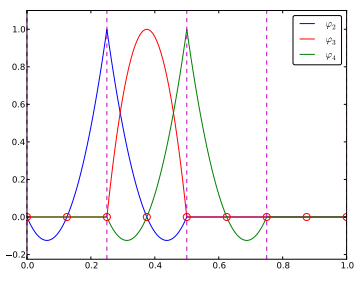
\includegraphics[width=0.7\linewidth]{img_18}
		\caption{Illustration of the piecewise quadratic basis functions associated
			with nodes in element 1.}
		\label{fig:img_18}
	\end{figure}
	
	\noindent Since $A_{i, j}$ is the integral of $\varphi_{i} \varphi_{j}$ it means that \textit{most of the elements in the coefficient matrix will be zero}. We will come back to these properties and use them actively in computations to save memory and CPU time.
	
	We let each element have $d+1$ nodes, resulting in local Lagrange polynomials of degree $d$. It is not a requirement to have the same $d$ value in each element, but for now we will assume so.
	\section[Example on piecewise quadratic finite element functions]{Example on piecewise quadratic finite element functions}
	\label{sec:sec_3_3}
	\noindent Figure 18 illustrates how piecewise quadratic basis functions can look like $(d=2)$. We work with the domain $\Omega=[0,1]$ divided into four equal-sized elements, each having three nodes. The \mycode{nodes} and \mycode{elements} lists in this particular example become
	\begin{lstlisting}[numbers=none]
		nodes = [0, 0.125, 0.25, 0.375, 0.5, 0.625, 0.75, 0.875, 1.0]
		elements = [[0, 1, 2], [2, 3, 4], [4, 5, 6], [6, 7, 8]]	
	\end{lstlisting}
	Figure \hyperref[fig:img_19]{19} sketches the mesh and the numbering. Nodes are marked with circles on the $x$ axis and element boundaries are marked with vertical dashed lines in Figure \hyperref[fig:img_18]{18}.
	
	Let us explain in detail how the basis functions are constructed according to the principles. Consider element number 1 in Figure \hyperref[fig:img_18]{18} $, \Omega^{(1)}=[0.25,0.5]$,
	\begin{figure}[H]
		\centering
		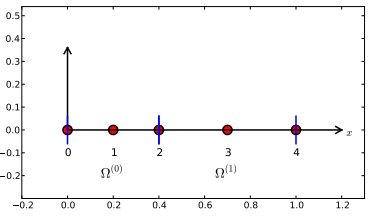
\includegraphics[width=0.7\linewidth]{img_19}
		\caption{Sketch of mesh with 4 elements and 3 nodes per element.}
		\label{fig:img_19}
	\end{figure}
	\noindent with local nodes 0,1 , and 2 corresponding to global nodes 2 , 3 , and 4 . The coordinates of these nodes are $0.25,0.375$, and $0.5$, respectively. We define three Lagrange polynomials on this element:
	\begin{enumerate}
		\item The polynomial that is 1 at local node $1(x=0.375$, global node 3 ) makes up the basis function $\varphi_{3}(x)$ over this element, with $\varphi_{3}(x)=0$ outside the element.
		\item The Lagrange polynomial that is 1 at local node 0 is the "right part" of the global basis function $\varphi_{2}(x)$. The "left part" of $\varphi_{2}(x)$ consists of a Lagrange polynomial associated with local node 2 in the neighboring element $\Omega^{(0)}=[0,0.25]$.
		\item Finally, the polynomial that is 1 at local node 2 (global node 4 ) is the "left part" of the global basis function $\varphi_{4}(x)$. The "right part" comes from the Lagrange polynomial that is 1 at local node 0 in the neighboring element $\Omega^{(2)}=[0.5,0.75]$.
	\end{enumerate}	
	
	\noindent As mentioned earlier, any global basis function $\varphi_{i}(x)$ is zero on elements that do not contain the node with global node number $i$.
	
	The other global functions associated with internal nodes, $\varphi_{1}, \varphi_{5}$, and $\varphi_{7}$, are all of the same shape as the drawn $\varphi_{3}$, while the global basis functions associated with shared nodes also have the same shape, provided the elements are of the same length.
	
	\section[Example on piecewise linear finite element functions]{Example on piecewise linear finite element functions}
	\label{sec:sec_3_4}
	Figure \hyperref[fig:img_20]{20} shows piecewise linear basis functions $(d=1)$. Also here we have four elements on $\Omega=[0,1]$. Consider the element $\Omega^{(1)}=[0.25,0.5]$. Now there are no internal nodes in the elements so that all basis functions are associated with nodes at the element boundaries and hence made up of two Lagrange
	\begin{figure}[H]
		\centering
		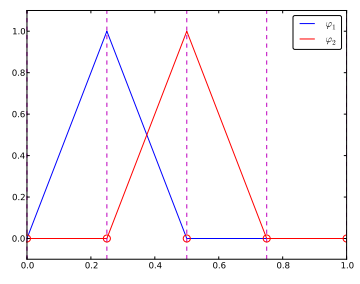
\includegraphics[width=0.7\linewidth]{img_20}
		\caption{Illustration of the piecewise linear basis functions associated with
			nodes in element 1.}
		\label{fig:img_20}
	\end{figure}
	
	\noindent polynomials from neighboring elements. For example, $\varphi_{1}(x)$ results from the Lagrange polynomial in element 0 that is 1 at local node 1 and 0 at local node 0 , combined with the Lagrange polynomial in element 1 that is 1 at local node 0 and 0 at local node 1 . The other basis functions are constructed similarly.
	
	Explicit mathematical formulas are needed for $\varphi_{i}(x)$ in computations. In the piecewise linear case, one can show that
	\begin{equation}\label{eqa53}
		\varphi_{i}(x)= \begin{cases}0, & x<x_{i-1}, \\ \left(x-x_{i-1}\right) /\left(x_{i}-x_{i-1}\right), & x_{i-1} \leq x<x_{i}, \\ 1-\left(x-x_{i}\right) /\left(x_{i+1}-x_{i}\right), & x_{i} \leq x<x_{i+1}, \\ 0, & x \geq x_{i+1}.\end{cases}
	\end{equation}
	Here, $x_{j}, j=i-1, i, i+1$, denotes the coordinate of node $j$. For elements of equal length $h$ the formulas can be simplified to
	\begin{equation}\label{eqa54}
		\varphi_{i}(x)= \begin{cases}0, & x<x_{i-1}, \\ \left(x-x_{i-1}\right) / h, & x_{i-1} \leq x<x_{i}, \\ 1-\left(x-x_{i}\right) / h, & x_{i} \leq x<x_{i+1}, \\ 0, & x \geq x_{i+1}\end{cases}
	\end{equation}
	\section[Example on piecewise cubic finite element basis functions]{Example on piecewise cubic finite element basis functions}
	\label{sec:sec_3_5}
	Piecewise cubic basis functions can be defined by introducing four nodes per element. Figure \hyperref[fig:img_21]{21} shows examples on $\varphi_{Wi}(x)$, $i=3,4,5,6$, associated with element number 1. Note that $\varphi_{4}$ and $\varphi_{5}$ are nonzero on element number 1 , while $\varphi_{3}$ and $\varphi_{6}$ are made up of Lagrange polynomials on two neighboring elements.
	\begin{figure}[H]
		\centering
		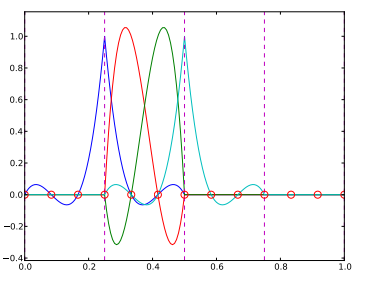
\includegraphics[width=0.7\linewidth]{img_21}
		\caption{Illustration of the piecewise cubic basis functions associated with
			nodes in element 1.}
		\label{fig:img_21}
	\end{figure}
	
	We see that all the piecewise linear basis functions have the same "hat" shape.
	They are naturally referred to as \textit{hat functions}, also called \textit{chapeau functions.}
	The piecewise quadratic functions in Figure \hyperref[fig:img_18]{18} are seen to be of two types.
	"Rounded hats" associated with internal nodes in the elements and some more
	"sombrero" shaped hats associated with element boundary nodes. Higher-order
	basis functions also have hat-like shapes, but the functions have pronounced
	oscillations in addition, as illustrated in Figure \hyperref[fig:img_21]{21}.
	
	A common terminology is to speak about \textit{linear elements} as elements with two
	local nodes associated with piecewise linear basis functions. Similarly, \textit{quadratic
		elements} and \textit{cubic elements} refer to piecewise quadratic or cubic functions
	over elements with three or four local nodes, respectively. Alternative names,
	frequently used later, are P1 elements for linear elements, P2 for quadratic
	elements, and so forth: Pd signifies degree d of the polynomial basis functions.
	
	\section[Calculating the linear system]{Calculating the linear system}
	\label{sec:sec_3_6}
	The elements in the coefficient matrix and right-hand side are given by the formulas (\hyperref[eqa27]{27}) and (\hyperref[eqa28]{28}), but now the choice of $\psi_{i}$ is $\varphi_{i}$. Consider P1 elements where $\varphi_{i}(x)$ piecewise linear. Nodes and elements numbered consecutively from left to right in a uniformly partitioned mesh imply the nodes
	$$
	x_{i}=i h, \quad i=0, \ldots, N,
	$$
	and the elements
	\begin{equation}\label{eqa55}
		\Omega^{(i)}=\left[x_{i}, x_{i+1}\right]=[i h,(i+1) h], \quad i=0, \ldots, N_{e}=N-1.
	\end{equation}
	We have in this case $N$ elements and $N+1$ nodes, and $\Omega=\left[x_{0}, x_{N}\right]$. The formula for $\varphi_{i}(x)$ is given by (\hyperref[eqa54]{54}) and a graphical illustration is provided in Figures \hyperref[fig:img_20]{20} and \hyperref[fig:img_23]{23} . First we clearly see from the figures the very important property $\varphi_{i}(x) \varphi_{j}(x) \neq 0$ if and only if $j=i-1, j=i$, or $j=i+1$, or alternatively expressed, if and only if $i$ and $j$ are nodes in the same element. Otherwise, $\varphi_{i}$ and $\varphi_{j}$ are too distant to have an overlap and consequently their product vanishes.
	\begin{figure}[H]
		\centering
		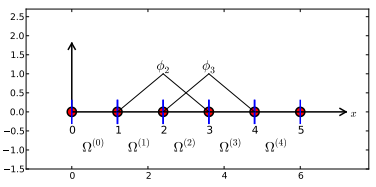
\includegraphics[width=0.7\linewidth]{img_22}
		\caption{Illustration of the piecewise linear basis functions corresponding to
			global node 2 and 3.}
		\label{fig:img_22}
	\end{figure}
	
	\noindent \textbf{Calculating a specific matrix entry.} Let us calculate the specific matrix entry $A_{2,3}=\int_{\Omega} \varphi_{2} \varphi_{3} \mathrm{~d} x$. Figure \hyperref[fig:img_22]{22} shows how $\varphi_{2}$ and $\varphi_{3}$ look like. We realize from this figure that the product $\varphi_{2} \varphi_{3} \neq 0$ only over element 2 , which contains node 2 and 3. The particular formulas for $\varphi_{2}(x)$ and $\varphi_{3}(x)$ on $\left[x_{2}, x_{3}\right]$ are found from (\hyperref[eqa54]{54}). The function $\varphi_{3}$ has positive slope over $\left[x_{2}, x_{3}\right]$ and corresponds to the interval $\left[x_{i-1}, x_{i}\right]$ in (\hyperref[eqa54]{54}). With $i=3$ we get
	$$
	\varphi_{3}(x)=\left(x-x_{2}\right) / h,
	$$
	while $\varphi_{2}(x)$ has negative slope over $\left[x_{2}, x_{3}\right]$ and corresponds to setting $i=2$ in (\hyperref[eqa54]{54}).
	
	$$
	\varphi_{2}(x)=1-\left(x-x_{2}\right) / h .
	$$
	We can now easily integrate,
	$$
	A_{2,3}=\int_{\Omega} \varphi_{2} \varphi_{3} \mathrm{~d} x=\int_{x_{2}}^{x_{3}}\left(1-\frac{x-x_{2}}{h}\right) \frac{x-x_{2}}{h} \mathrm{~d} x=\frac{h}{6}.
	$$
	The diagonal entry in the coefficient matrix becomes
	$$
	A_{2,2}=\int_{x_{1}}^{x_{2}}\left(\frac{x-x_{1}}{h}\right)^{2} \mathrm{~d} x+\int_{x_{2}}^{x_{3}}\left(1-\frac{x-x_{2}}{h}\right)^{2} \mathrm{~d} x=\frac{h}{3}.
	$$
	The entry $A_{2,1}$ has an the integral that is geometrically similar to the situation in Figure \hyperref[fig:img_22]{22}, so we get $A_{2,1}=h / 6$.
	\bigbreak
	\noindent \textbf{Calculating a general row in the matrix.} We can now generalize the calculation of matrix entries to a general row number $i$. The entry $A_{i, i-1}=$ $\int_{\Omega} \varphi_{i} \varphi_{i-1} \mathrm{~d} x$ involves hat functions as depicted in Figure \hyperref[fig:img_23]{23} . Since the integral is geometrically identical to the situation with specific nodes 2 and 3 , we realize that $A_{i, i-1}=A_{i, i+1}=h / 6$ and $A_{i, i}=2 h / 3$. However, we can compute the integral directly too:
	$$
	\begin{aligned}
		A_{i, i-1} &=\int_{\Omega} \varphi_{i} \varphi_{i-1} \mathrm{~d} x \\
		&=\underbrace{\int_{x_{i-2}}^{x_{i-1}} \varphi_{i} \varphi_{i-1} \mathrm{~d} x}_{\varphi_{i}=0}+\int_{x_{i-1}}^{x_{i}} \varphi_{i} \varphi_{i-1} \mathrm{~d} x+\underbrace{\int_{x_{i}}^{x_{i+1}} \varphi_{i} \varphi_{i-1} \mathrm{~d} x}_{\varphi_{i-1}=0} \\
		&=\int_{x_{i-1}}^{x_{i}} \underbrace{\left(\frac{x-x_{i}}{h}\right)}_{\varphi_{i}(x)} \underbrace{\left(1-\frac{x-x_{i-1}}{h}\right)}_{\varphi_{i-1}(x)} \mathrm{d} x=\frac{h}{6}.
	\end{aligned}
	$$
	The particular formulas for $\varphi_{i-1}(x)$ and $\varphi_{i}(x)$ on $\left[x_{i-1}, x_{i}\right]$ are found from (\hyperref[eqa54]{54}): $\varphi_{i}$ is the linear function with positive slope, corresponding to the interval $\left[x_{i-1}, x_{i}\right]$ in (\hyperref[eqa54]{54}), while $\phi_{i-1}$ has a negative slope so the definition in interval $\left[x_{i}, x_{i+1}\right]$ in (\hyperref[eqa54]{54}) must be used. (The appearance of $i$ in (\hyperref[eqa54]{54}) and the integral might be confusing, as we speak about two different $i$ indices.)
	
	The first and last row of the coefficient matrix lead to slightly different integrals:
	$$
	A_{0,0}=\int_{\Omega} \varphi_{0}^{2} \mathrm{~d} x=\int_{x_{0}}^{x_{1}}\left(1-\frac{x-x_{0}}{h}\right)^{2} \mathrm{~d} x=\frac{h}{3}.
	$$
	Similarly, $A_{N, N}$ involves an integral over only one element and equals hence $h / 3$. The general formula for $b_{i}$, see Figure \hyperref[fig:img_24]{24}, is now easy to set up
	\begin{figure}[H]
		\centering
		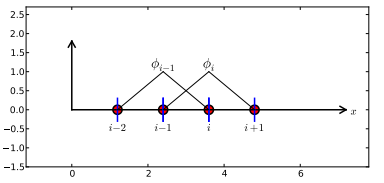
\includegraphics[width=0.7\linewidth]{img_23}
		\caption{Illustration of two neighboring linear (hat) functions with general
			node numbers.}
		\label{fig:img_23}
	\end{figure}
	\begin{figure}[H]
		\centering
		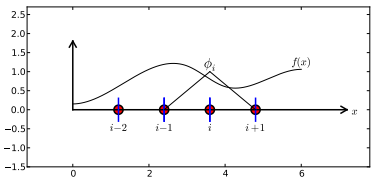
\includegraphics[width=0.7\linewidth]{img_24}
		\caption{Right-hand side integral with the product of a basis function and
			the given function to approximate.}
		\label{fig:img_24}
	\end{figure}
	\begin{equation}\label{eqa56}
		b_{i}=\int_{\Omega} \varphi_{i}(x) f(x) \mathrm{d} x=\int_{x_{i-1}}^{x_{i}} \frac{x-x_{i-1}}{h} f(x) \mathrm{d} x+\int_{x_{i}}^{x_{i+1}}\left(1-\frac{x-x_{i}}{h}\right) f(x) \mathrm{d} x.
	\end{equation}
	We need a specific $f(x)$ function to compute these integrals. With two equal-sized elements in $\Omega=[0,1]$ and $f(x)=x(1-x)$, one gets
	$$
	A=\frac{h}{6}\left(\begin{array}{ccc}
		2 & 1 & 0 \\
		1 & 4 & 1 \\
		0 & 1 & 2
	\end{array}\right), \quad b=\frac{h^{2}}{12}\left(\begin{array}{c}
		2-3 h \\
		12-14 h \\
		10-17 h
	\end{array}\right)
	$$
	The solution becomes
	$$
	c_{0}=\frac{h^{2}}{6}, \quad c_{1}=h-\frac{5}{6} h^{2}, \quad c_{2}=2 h-\frac{23}{6} h^{2}.
	$$
	The resulting function
	$$
	u(x)=c_{0} \varphi_{0}(x)+c_{1} \varphi_{1}(x)+c_{2} \varphi_{2}(x)
	$$
	is displayed in Figure \hyperref[fig:img_25]{25} (left). Doubling the number of elements to four leads to the improved approximation in the right part of Figure \hyperref[fig:img_25]{25} .
	\begin{figure}[H]
		\centering
		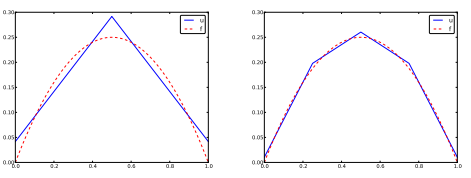
\includegraphics[width=0.7\linewidth]{img_25}
		\caption{Least squares approximation of a parabola using 2 (left) and 4
			(right) P1 elements.}
		\label{fig:img_25}
	\end{figure}
	
	\section[Assembly of elementwise computations]{Assembly of elementwise computations}
	\label{sec:sec_3_7}
	The integrals above are naturally split into integrals over individual elements since the formulas change with the elements. This idea of splitting the integral is fundamental in all practical implementations of the finite element method.
	Let us split the integral over $\Omega$ into a sum of contributions from each element:
	\begin{equation}\label{eqa57}
		A_{i, j}=\int_{\Omega} \rho_{i} \rho_{j} \mathrm{~d} x=\sum_{e} A_{i, j}^{(e)}, \quad A_{i, j}^{(e)}=\int_{\Omega^{(e)}} \rho_{i} \rho_{j} \mathrm{~d} x.
	\end{equation}
	Now, $A_{i, j}^{(e)} \neq 0$ if and only if $i$ and $j$ are nodes in element $e$. Introduce $i=q(e, r)$ as the mapping of local node number $r$ in element $e$ to the global node number $i$. This is just a short mathematical notation for the expression $i=e l$ ements [e] [r] in a program. Let $r$ and $s$ be the local node numbers corresponding to the global node numbers $i=q(e, r)$ and $j=q(e, s)$. With $d$ nodes per element, all the nonzero elements in $A_{i, j}^{(e)}$ arise from the integrals involving basis functions with indices corresponding to the global node numbers in element number $e$ :
	$$
	\int_{\Omega^{(e)}} \varphi_{q(e, r)} \varphi_{q(e, s)} \mathrm{d} x, \quad r, s=0, \ldots, d .
	$$
	These contributions can be collected in a $(d+1) \times(d+1)$ matrix known as the \textit{element matrix}. Let $I_{d}=\{0, \ldots, d\}$ be the valid indices of $r$ and $s$. We introduce the notation
	$$
	\tilde{A}^{(e)}=\left\{\tilde{A}_{r, s}^{(e)}\right\}, \quad r, s \in I_{d},
	$$
	for the element matrix. For the case $d=2$ we have
	$$
	\tilde{A}^{(e)}=\left[\begin{array}{ccc}
		\tilde{A}_{0,0}^{(e)} & \tilde{A}_{0,1}^{(e)} & \tilde{A}_{0,2}^{(e)} \\
		\tilde{A}_{1,0}^{(e)} & \tilde{A}_{1,1}^{(e)} & \tilde{A}_{1,2}^{(e)} \\
		\tilde{A}_{2,0}^{(e)} & \tilde{A}_{2,1}^{(e)} & \tilde{A}_{2,2}^{(e)}
	\end{array}\right] .
	$$
	Given the numbers $\tilde{A}_{r, s}^{(e)}$, we should according to (\hyperref[eqa57]{57}) add the contributions to the global coefficient matrix by
	\begin{equation}\label{eqa58}
		A_{q(e, r), q(e, s)}:=A_{q(e, r), q(e, s)}+\tilde{A}_{r, s}^{(e)}, \quad r, s \in I_{d} .
	\end{equation}
	
	This process of adding in elementwise contributions to the global matrix is called \textit{finite element assembly} or simply \textit{assembly}. Figure \hyperref[fig:img_26]{26} illustrates how element matrices for elements with two nodes are added into the global matrix. More specifically, the figure shows how the element matrix associated with elements 1 and 2 assembled, assuming that global nodes are numbered from left to right in the domain. With regularly numbered P3 elements, where the element matrices have size $4 \times 4$, the assembly of elements 1 and 2 are sketched in Figure \hyperref[fig:img_27]{27}.
	\begin{figure}[H]
		\centering
		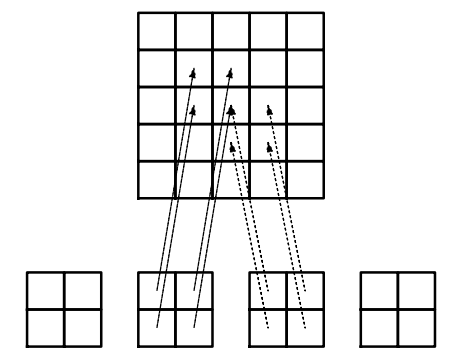
\includegraphics[width=0.7\linewidth]{img_26}
		\caption{Illustration of matrix assembly: regularly numbered P1 elements.}
		\label{fig:img_26}
	\end{figure}
	
	After assembly of element matrices corresponding to regularly numbered
	elements and nodes are understood, it is wise to study the assembly process for
	irregularly numbered elements and nodes. Figure \hyperref[fig:img_17]{17} shows a mesh where the
	elements array, or q(e, r) mapping in mathematical notation, is given as
	\begin{figure}[H]
		\centering
		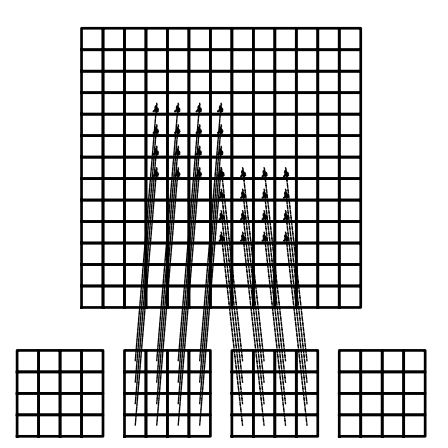
\includegraphics[width=0.7\linewidth]{img_27}
		\caption{Illustration of matrix assembly: regularly numbered P3 elements.}
		\label{fig:img_27}
	\end{figure}
	
	\begin{lstlisting}[numbers=none]
		elements = [[2, 1], [4, 5], [0, 4], [3, 0], [5, 2]
	\end{lstlisting}
	The associated assembly of element matrices 1 and 2 is sketched in Figure \hyperref[fig:img_28]{28}. 
	
	These three assembly processes can also be \href{http://hplgit.github.io/INF5620/doc/pub/mov-fem/fe_assembly.html}{animated.}
	
	
	The right-hand side of the linear system is also computed elementwise:
	\begin{equation}\label{eqa59}
		b_{i}=\int_{\Omega} f(x) \varphi_{i}(x) \mathrm{d} x=\sum_{e} b_{i}^{(e)}, \quad b_{i}^{(e)}=\int_{\Omega^{(e)}} f(x) \varphi_{i}(x) \mathrm{d} x.
	\end{equation}
	We observe that $b_{i}^{(e)} \neq 0$ if and only if global node $i$ is a node in element $e$. With $d$ nodes per element we can collect the $d+1$ nonzero contributions $b_{i}^{(e)}$, for $i=q(e, r), r \in I_{d}$, in an \textit{element vector}
	$$
	\tilde{b}_{r}^{(e)}=\left\{\tilde{b}_{r}^{(e)}\right\}, \quad r \in I_{d} .
	$$
	These contributions are added to the global right-hand side by an assembly process similar to that for the element matrices:
	\begin{figure}[H]
		\centering
		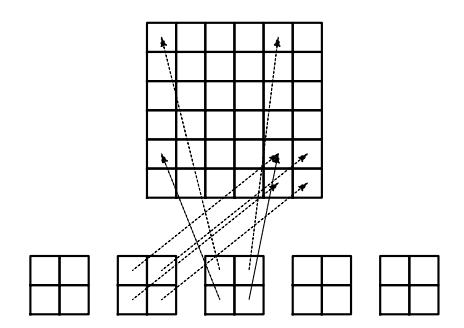
\includegraphics[width=0.7\linewidth]{img_28}
		\caption{Illustration of matrix assembly: irregularly numbered P1 elements.}
		\label{fig:img_28}
	\end{figure}
	\begin{equation}\label{eqa60}
		b_{q(e, r)}:=b_{q(e, r)}+\tilde{b}_{r}^{(e)}, \quad r \in I_{d}.
	\end{equation}
	\section[Mapping to a reference element]{Mapping to a reference element}
	\label{sec:sec_3_8}
	Instead of computing the integrals
	$$
	\tilde{A}_{r, s}^{(e)}=\int_{\Omega^{(e)}} \varphi_{q(e, r)}(x) \varphi_{q(e, s)}(x) \mathrm{d} x
	$$
	over some element $\Omega^{(e)}=\left[x_{L}, x_{R}\right]$, it is convenient to map the element domain $\left[x_{L}, x_{R}\right]$ to a standardized reference element domain $[-1,1]$. (We have now introduced $x_{L}$ and $x_{R}$ as the left and right boundary points of an arbitrary element. With a natural, regular numbering of nodes and elements from left to right through the domain, we have $x_{L}=x_{e}$ and $x_{R}=x_{e+1}$ for $\mathrm{P} 1$ elements.)
	
	Let $X \in[-1,1]$ be the coordinate in the reference element. A linear or \textit{affine mapping} from $X$ to $x$ reads
	\begin{equation}\label{eqa61}
		x=\frac{1}{2}\left(x_{L}+x_{R}\right)+\frac{1}{2}\left(x_{R}-x_{L}\right) X.
	\end{equation}
	This relation can alternatively be expressed by
	\begin{equation}\label{eqa62}
		x=x_{m}+\frac{1}{2} h X,
	\end{equation}
	where we have introduced the element midpoint $x_{m}=\left(x_{L}+x_{R}\right) / 2$ and the element length $h=x_{R}-x_{L}$.
	
	Integrating on the reference element is a matter of just changing the integration variable from $x$ to $X$. Let
	\begin{equation}\label{eqa63}
		\tilde{\varphi}_{r}(X)=\varphi_{q(e, r)}(x(X))
	\end{equation}
	be the basis function associated with local node number $r$ in the reference element. The integral transformation reads
	\begin{equation}\label{eqa64}
		\tilde{A}_{r, s}^{(e)}=\int_{\Omega^{(e)}} \varphi_{q(e, r)}(x) \varphi_{q(e, s)}(x) \mathrm{d} x=\int_{-1}^{1} \tilde{\varphi}_{r}(X) \tilde{\varphi}_{s}(X) \frac{d x}{d X} \mathrm{~d} X.
	\end{equation}
	The stretch factor $d x / d X$ between the $x$ and $X$ coordinates becomes the determinant of the Jacobian matrix of the mapping between the coordinate systems in $2 \mathrm{D}$ and 3D. To obtain a uniform notation for $1 \mathrm{D}, 2 \mathrm{D}$, and 3D problems we therefore replace $d x / d X$ by det $J$ already now. In $1 \mathrm{D}$, $\operatorname{det} J=d x / d X=h / 2$. The integration over the reference element is then written as
	\begin{equation}\label{eqa65}
		\tilde{A}_{r, s}^{(e)}=\int_{-1}^{1} \tilde{\varphi}_{r}(X) \tilde{\varphi}_{s}(X) \operatorname{det} J d X.
	\end{equation}
	The corresponding formula for the element vector entries becomes
	\begin{equation}\label{eqa66}
		\tilde{b}_{r}^{(e)}=\int_{\Omega^{(e)}} f(x) \varphi_{q(e, r)}(x) d x=\int_{-1}^{1} f(x(X)) \tilde{\varphi}_{r}(X) \operatorname{det} J d X.
	\end{equation}
	
	Since we from now on will work in the reference element, we need explicit mathematical formulas for the basis functions $\varphi_{i}(x)$ in the reference element only, i.e., we only need to specify formulas for $\tilde{\varphi}_{r}(X)$. This is a very convenient simplification compared to specifying piecewise polynomials in the physical domain.
	
	The $\tilde{\varphi}_{r}(x)$ functions are simply the Lagrange polynomials defined through the local nodes in the reference element. For $d=1$ and two nodes per element, we have the linear Lagrange polynomials
	\begin{equation}\label{eqa67}
		\tilde{\varphi}_{0}(X) =\frac{1}{2}(1-X)
	\end{equation}
	\begin{equation}\label{eqa68}
		\tilde{\varphi}_{1}(X) =\frac{1}{2}(1+X)
	\end{equation}
	Quadratic polynomials, $d=2$, have the formulas
	\begin{equation}\label{eqa69}
		\tilde{\varphi}_{0}(X) =\frac{1}{2}(X-1) X
	\end{equation}
	\begin{equation}\label{eqa70}
		\tilde{\varphi}_{1}(X) =1-X^{2}
	\end{equation}
	\begin{equation}\label{eqa71}
		\tilde{\varphi}_{2}(X) =\frac{1}{2}(X+1)X
	\end{equation}
	In general,
	\begin{equation}\label{eqa72}
		\tilde{\varphi}_{r}(X)=\prod_{s=0, s \neq r}^{d} \frac{X-X_{(s)}}{X_{(r)}-X_{(s)}},
	\end{equation}
	where $X_{(0)}, \ldots, X_{(d)}$ are the coordinates of the local nodes in the reference element. These are normally uniformly spaced: $X_{(r)}=-1+2 r / d, r \in I_{d}$.
	\begin{mybox}
		\textbf{Why reference elements?}
		
		\noindent The great advantage of using reference elements is that the formulas for the basis functions, $\tilde{\varphi}_{r}(X)$, are the same for all elements and independent of the element geometry (length and location in the mesh). The geometric information is "factored out" in the simple mapping formula and the associated det $J$ quantity, but this information is (here taken as) the same for element types. Also, the integration domain is the same for all elements.
	\end{mybox}
	
	
	\section[Example: Integration over a reference element]{Example: Integration over a reference element}
	\label{sec:sec_3_9}
	\noindent To illustrate the concepts from the previous section in a specific example, we now consider calculation of the element matrix and vector for a specific choice of $d$ and $f(x)$. A simple choice is $d=1$ (P1 elements) and $f(x)=x(1-x)$ on $\Omega=[0,1]$. We have the general expressions (\hyperref[eqa65]{65}) and (\hyperref[eqa66]{66}) for $\tilde{A}_{r, s}^{(e)}$ and $\tilde{b}_{r}^{(e)}$. Writing these out for the choices (\hyperref[eqa67]{67}) and (\hyperref[eqa68]{68}), and using that $\operatorname{det} J=h / 2$, we can do the following calculations of the element matrix entries:
	\begin{equation}\label{eqa73}
		\begin{aligned}
			\tilde{A}_{0,0}^{(e)} &=\int_{-1}^{1} \tilde{\varphi}_{0}(X) \tilde{\varphi}_{0}(X) \frac{h}{2} d X \\
			&=\int_{-1}^{1} \frac{1}{2}(1-X) \frac{1}{2}(1-X) \frac{h}{2} d X=\frac{h}{8} \int_{-1}^{1}(1-X)^{2} d X=\frac{h}{3},
		\end{aligned}
	\end{equation}
	\begin{equation}\label{eqa74}
		\begin{aligned}
			\tilde{A}_{1,0}^{(e)} &=\int_{-1}^{1} \tilde{\varphi}_{1}(X) \tilde{\varphi}_{0}(X) \frac{h}{2} d X \\
			&=\int_{-1}^{1} \frac{1}{2}(1+X) \frac{1}{2}(1-X) \frac{h}{2} d X=\frac{h}{8} \int_{-1}^{1}\left(1-X^{2}\right) d X=\frac{h}{6},
		\end{aligned}
	\end{equation}
	\begin{equation}\label{eqa75}
		\tilde{A}_{0,1}^{(e)} =\tilde{A}_{1,0}^{(e)},
	\end{equation}
	\begin{equation}\label{eqa76}
		\begin{aligned}
			\tilde{A}_{1,1}^{(e)} &=\int_{-1}^{1} \tilde{\varphi}_{1}(X) \tilde{\varphi}_{1}(X) \frac{h}{2} d X \\
			&=\int_{-1}^{1} \frac{1}{2}(1+X) \frac{1}{2}(1+X) \frac{h}{2} d X=\frac{h}{8} \int_{-1}^{1}(1+X)^{2} d X=\frac{h}{3}.
		\end{aligned}
	\end{equation}
	The corresponding entries in the element vector becomes
	\begin{equation}\label{eqa77}
		\begin{aligned}
			\tilde{b}_{0}^{(e)} &=\int_{-1}^{1} f(x(X)) \tilde{\varphi}_{0}(X) \frac{h}{2} d X \\
			&=\int_{-1}^{1}\left(x_{m}+\frac{1}{2} h X\right)\left(1-\left(x_{m}+\frac{1}{2} h X\right)\right) \frac{1}{2}(1-X) \frac{h}{2} d X \\
			&=-\frac{1}{24} h^{3}+\frac{1}{6} h^{2} x_{m}-\frac{1}{12} h^{2}-\frac{1}{2} h x_{m}^{2}+\frac{1}{2} h x_{m}.
		\end{aligned}
	\end{equation}
	\begin{equation}\label{eqa78}
		\begin{aligned}
			\tilde{b}_{1}^{(e)} &=\int_{-1}^{1} f(x(X)) \tilde{\varphi}_{1}(X) \frac{h}{2} d X \\
			&=\int_{-1}^{1}\left(x_{m}+\frac{1}{2} h X\right)\left(1-\left(x_{m}+\frac{1}{2} h X\right)\right) \frac{1}{2}(1+X) \frac{h}{2} d X \\
			&=-\frac{1}{24} h^{3}-\frac{1}{6} h^{2} x_{m}+\frac{1}{12} h^{2}-\frac{1}{2} h x_{m}^{2}+\frac{1}{2} h x_{m}.
		\end{aligned}
	\end{equation}
	In the last two expressions we have used the element midpoint $x_{m}$.
	
	Integration of lower-degree polynomials above is tedious, and higher-degree polynomials involve very much more algebra, but \mycode{sympy} may help. For example, we can easily calculate (\hyperref[eqa73]{73}), (\hyperref[eqa73]{73}) and (\hyperref[eqa77]{77}) by
	\begin{lstlisting}[numbers=none]
		>>> import sympy as sp
		>>> x, x_m, h, X = sp.symbols('x x_m h X')
		>>> sp.integrate(h/8*(1-X)**2, (X, -1, 1))
		h/3
		>>> sp.integrate(h/8*(1+X)*(1-X), (X, -1, 1))
		h/6
		>>> x = x_m + h/2*X
		>>> b_0 = sp.integrate(h/4*x*(1-x)*(1-X), (X, -1, 1))
		>>> print b_0
		-h**3/24 + h**2*x_m/6 - h**2/12 - h*x_m**2/2 + h*x_m/2	
	\end{lstlisting}
	For inclusion of formulas in documents (like the present one), \mycode{sympy} can print
	expressions in \mycode{LATEX} format:
	\begin{lstlisting}[numbers=none]
	>>> print sp.latex(b_0, mode='plain')
	- \frac{1}{24} h^{3} + \frac{1}{6} h^{2} x_{m}
	- \frac{1}{12} h^{2} - \half h x_{m}^{2}
	+ \half h x_{m
	\end{lstlisting}
\clearpage
\end{document} 
